%\documentclass{article}
%\usepackage{subfiles}
%\usepackage{forest}
%\usetikzlibrary{shadows,arrows.meta}
%\usepackage{float}
%\usepackage{colortbl}
%\usepackage{multirow}
%\usepackage{array}
%\usepackage{minted}
%\usepackage{longtable}

%\usepackage[
%backend=biber,
%style=authoryear,
%sorting=ynt
%]{biblatex}
%\addbibresource{refs.bib}

%A4 page size = 210mm, 297mm / inset total = size-margin
%\usepackage[a4paper, total={190mm, 277mm}]{geometry}
%\usepackage{fontspec}
%\setmainfont{TimesNewRoman}

%\title{}
%\author{}
%\begin{document}
\large
\subsection{Consolidated Risk Matrix}
\begin{table}[H]
    \centering
   % \renewcommand{\arraystretch}{3.5} % Adjust row height
    \begin{tabular}{ccc|m{0.5cm}|m{0.5cm}|m{0.5cm}|m{0.5cm}|m{0.5cm}|}
    %\begin{tabular}{ccc|m{2cm}|m{2cm}|m{2cm}|m{2cm}|m{2cm}|}
        \cline{4-8}
        \cline{4-8}
        \multirow{5}{*}{\rotatebox[origin=c]{90}{Likelihood}} & & 5 & \cellcolor{green!10}&  \cellcolor{yellow!10}& \cellcolor{red!10} & \cellcolor{red!10} L.1 & \cellcolor{red!10} P.2 \\
        \cline{4-8}
        &   &4  & \cellcolor{green!10}   &  \cellcolor{yellow!10}  &  \cellcolor{yellow!10} L.2  &  \cellcolor{red!10} P.1  & \cellcolor{red!10}\\
        \cline{4-8}
        &   & 3 & \cellcolor{green!10} & \cellcolor{yellow!10} & \cellcolor{yellow!10} & \cellcolor{yellow!10} & \cellcolor{red!10} M.1 \\
         \cline{4-8}
        & &2 & \cellcolor{green!10} & \cellcolor{green!10} L.3 & \cellcolor{green!10} M.3 & \cellcolor{yellow!10} M.2 & \cellcolor{yellow!10}\\
         \cline{4-8}
        & & 1& \cellcolor{green!10} & \cellcolor{green!10} & \cellcolor{green!10} P.4 & \cellcolor{green!10} P.3 & \cellcolor{yellow!10}\\
         \cline{4-8}
        & & \multicolumn{1}{c}{} & \multicolumn{1}{c}{1} & \multicolumn{1}{c}{2} & \multicolumn{1}{c}{3} & \multicolumn{1}{c}{4} &\multicolumn{1}{c}{5} \\
         & & \multicolumn{1}{c}{} & \multicolumn{1}{c}{} & \multicolumn{1}{c}{} & \multicolumn{1}{c}{} & \multicolumn{1}{c}{} &\multicolumn{1}{c}{} \\
         & & \multicolumn{1}{c}{} & \multicolumn{5}{c}{Consequence}
    \end{tabular}
     \caption{Risk matrix for the project}
    %\label{tab:risk_label}
\end{table}

\begin{longtable}{p{3cm}p{3cm} cc p{3cm}}
    \caption{Description and mitigation of risk present in Risk matrix }\\
    \centering
    
     
    %\begin{tabular}{p{3cm}p{3cm} cc p{3cm}}
        Risk & Description  & Consequence Level & Likelihood & Mitigation \\
        
         \hline
         \multicolumn{5}{c}{Production}\\
         \hline
         P.1 Financial & Risk caused by fluctuating material prices, insufficient cash flow, product recalls & 5 & 4 & Good financial planning and budgeting mitigates the risk. \\
         P.2 Operational & Equipment failure, supply chain disruptions and labour shortages, low quality production & 5 & 5 & Ensure backup machinery is available, have small back-up stock of raw materials, ensure good employee relations\\
         P.3 Natural disasters & Damage to property due to natural disasters & 4 & 1 & Have emergency funds available.\\
         P4. Cybersecurity & Cybersecurity threats that cause production outages and intellectual property theft & 3 & 1 & Ensure good cybersecurity practices and employee training\\
         \hline
         \multicolumn{5}{c}{Logistics}\\
         \hline
         L.1 Stockouts & Risk of insufficient stock due to JIT inventory system & 4 & 5 & Ensure good logistical planning and have a small back-up stock available.\\
         L.2 Supplier delays & Risk of production delays due to supplier delays & 3 & 4 & Account for possible suppliers delay when planning logistics\\
         L.3 Transit damage & Damage caused by transit & 2 & 2 & Ensure good protective packaging for outbound logistics.\\ 
         \hline
          %\newpage
          \caption{Description and mitigation of risk present in Risk matrix continued}\\
           Risk & Description  & Consequence Level & Likelihood & Mitigation \\
          \hline
         \multicolumn{5}{c}{Marketing}\\
         \hline
         M.1 Financial & Loss of revenue due to incorrect or misdirected marketing resulting in low return of investment & 5 & 3 & Good market research and good marketing strategy, avoids invective marketing\\
         M.2 Reputational & Loss of reputation due to bad marketing strategies & 4 & 2 & Good market research and strategy, as well as a test audience mitigates the risk\\
         M.3 Compliance & Risk of non-compliance with rule and regulations of Advertisement & 3 & 2 & Well trained employees and an experienced production componany avoids this risk.\\
         \hline
         \hline
         
    %\end{tabular}
   
    %\label{tab:my_risk_label}
\end{longtable}

\subsection{Business intelligence}

A simple linear regression model was implemented to predict the trend present in the CPI of South Africa (\cite{data}) for the next 10 years. Figure \ref{fig:reg_model} shows the model. The predicted values can be used to predict future costs of good and services required for business operations. It should be noted that the model only indicates the trend and should not be taken at face value, since future market volatility may overshoot or undershoot the prediction. Figure \ref{fig:code} shows the code used to obtain the model

\begin{figure}[H]
    \centering
    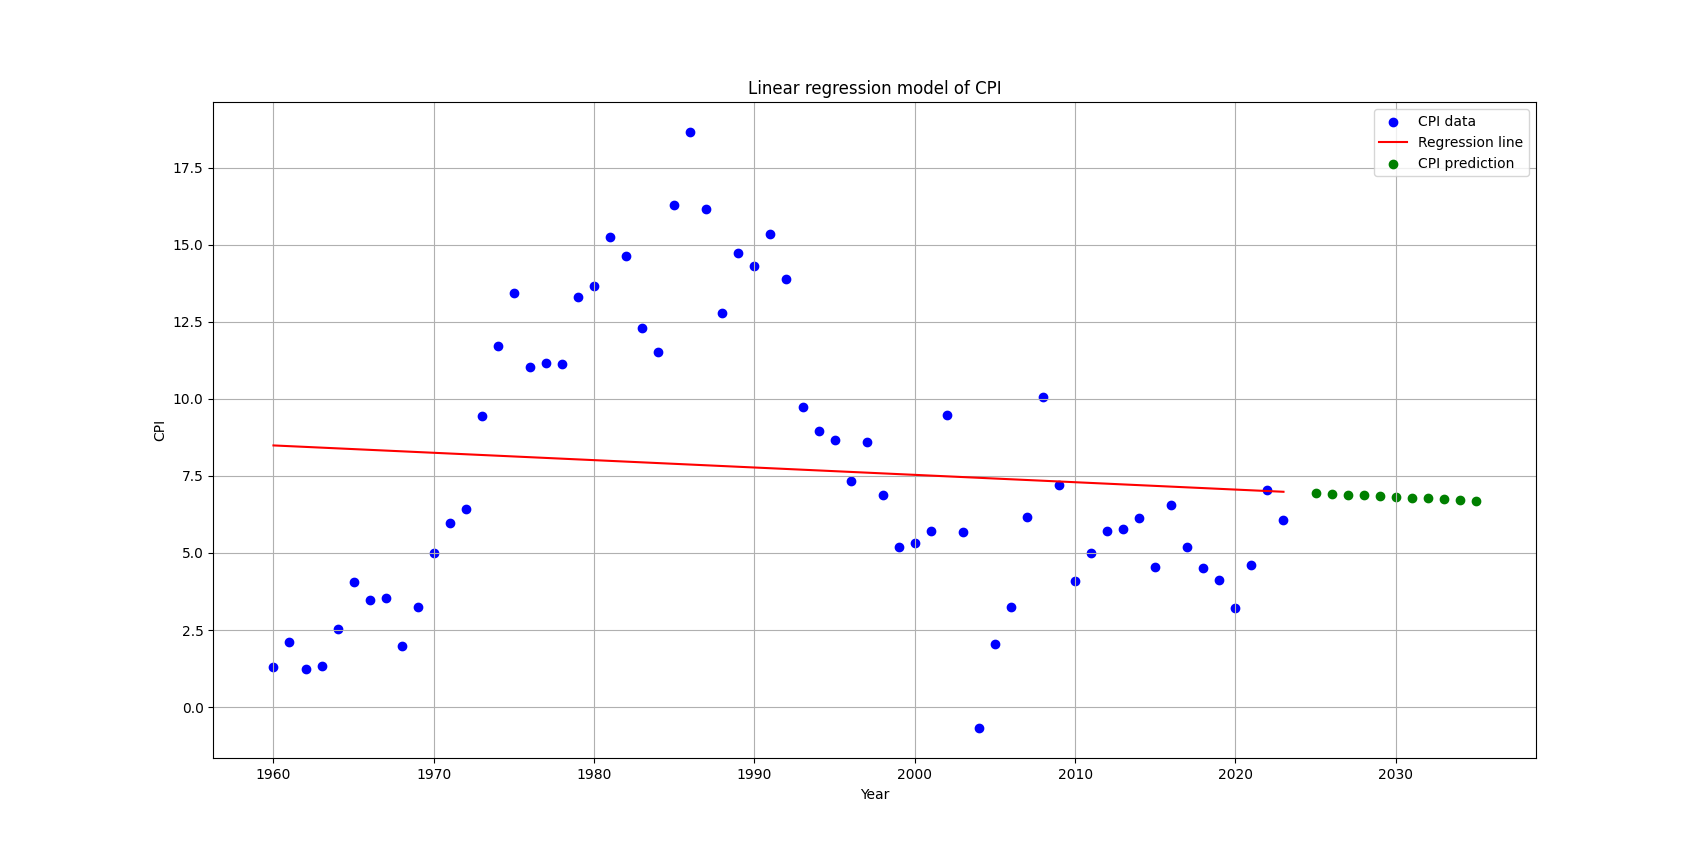
\includegraphics[width=0.75\linewidth]{figures/CPI_model.png}
    \caption{Linear regression model of CPI of South Africa}
    \label{fig:reg_model}
\end{figure}

\begin{table}[H]
    \centering
    \caption{Tabulation of the predicted CPI values}
    \begin{tabular}{cc|cc}
        Year&CPI & Year &CPI\\
        \hline
        2025&6.937&     2030&6.818\\
        2026&6.913&     2031&6.794\\
        2027&6.890&    2032&6.770\\
        2028&6.866&    2033&6.746\\
        2029&6.842&     2034&6.723\\
        \hline
        \hline

    \end{tabular}
    
    %\label{tab:cpi_predict}
\end{table}

\begin{figure}[H]
    \centering
   \inputminted[breaklines]{python}{figures/BI_model.py}

    \caption{Python code for linear regression model}
    \label{fig:code}
\end{figure}

%https://www.macrotrends.net/global-metrics/countries/zaf/south-africa/inflation-rate-cpi
%\printbibliography
%\end{document}
